\documentclass[tikz,border=5pt]{standalone}
\usepackage{amsmath,amssymb}
\usetikzlibrary{shapes.geometric, arrows.meta, positioning, calc, fit, backgrounds}

\begin{document}
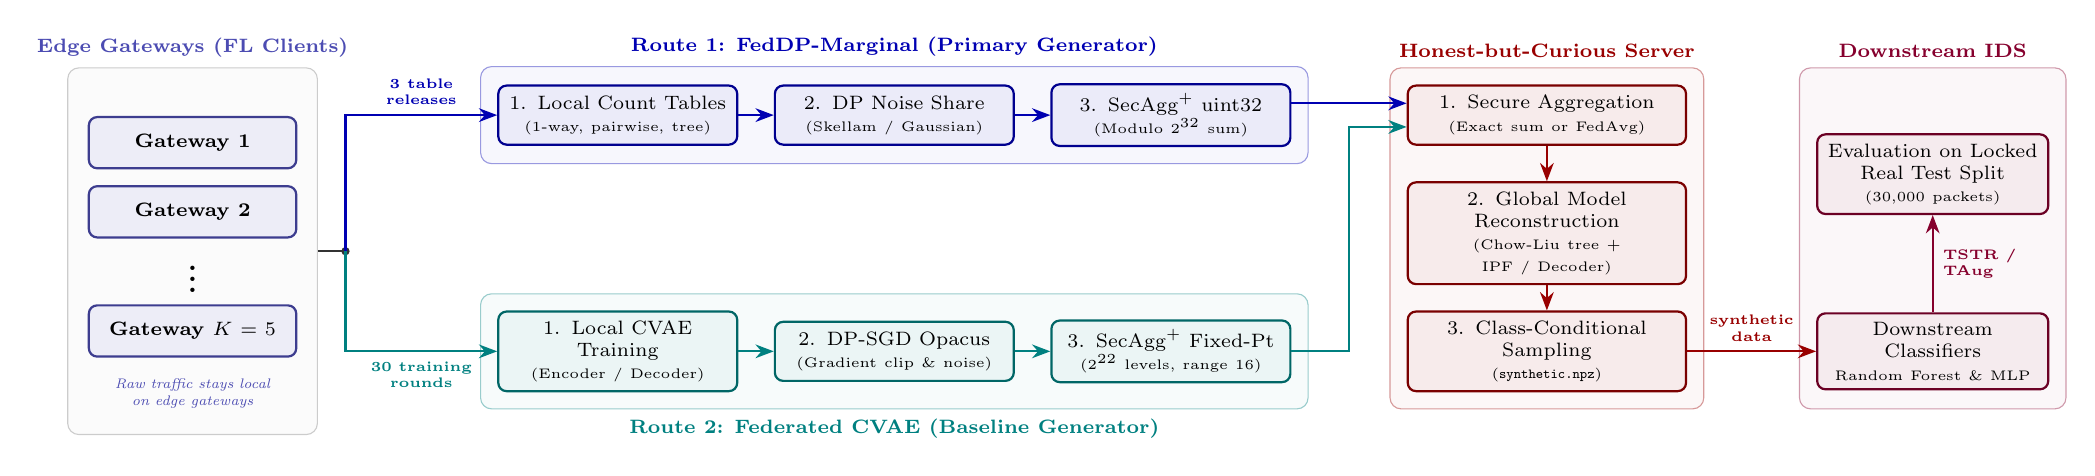
\begin{tikzpicture}[
    font=\scriptsize, >=Stealth,
    tier/.style={rectangle, draw=gray!40, fill=gray!3, rounded corners=4pt, inner sep=6pt},
    gwbox/.style={
        rectangle, draw=blue!40!gray!80!black, fill=blue!40!gray!10, rounded corners=3pt, thick,
        text width=2.4cm, minimum height=0.65cm, align=center, font=\scriptsize\bfseries
    },
    route1box/.style={
        rectangle, draw=blue!70!black!80!black, fill=blue!70!black!8, rounded corners=3pt, thick,
        text width=2.8cm, minimum height=0.75cm, align=center
    },
    route2box/.style={
        rectangle, draw=teal!80!black, fill=teal!8, rounded corners=3pt, thick,
        text width=2.8cm, minimum height=0.75cm, align=center
    },
    srvbox/.style={
        rectangle, draw=red!60!black!80!black, fill=red!60!black!8, rounded corners=3pt, thick,
        text width=3.3cm, minimum height=0.75cm, align=center
    },
    idsbox/.style={
        rectangle, draw=purple!70!black!80!black, fill=purple!70!black!8, rounded corners=3pt, thick,
        text width=2.7cm, minimum height=0.85cm, align=center
    },
    arr/.style={->, thick, draw=black!80}
]

% Define color aliases
\colorlet{slate}{blue!40!gray}
\colorlet{indigo}{blue!70!black}
\colorlet{crimson}{red!60!black}
\colorlet{violet}{purple!70!black}

% --- TIER 1: Edge Gateways ---
\node[gwbox] (g1) at (0, 1.15) {Gateway 1};
\node[gwbox] (g2) [below=0.2cm of g1] {Gateway 2};
\node[font=\bfseries] (gdots) [below=0.02cm of g2] {$\vdots$};
\node[gwbox] (gk) [below=0.02cm of gdots] {Gateway $K = 5$};
\node[text width=2.5cm, align=center, font=\tiny\itshape, text=slate] (gnote) [below=0.15cm of gk] {Raw traffic stays local\\on edge gateways};

% --- TIER 2: Dual Generator Routes ---
% Route 1 (Top lane)
\node[route1box] (r1_1) at (5.4, 1.5) {1. Local Count Tables\\{\tiny (1-way, pairwise, tree)}};
\node[route1box] (r1_2) [right=0.45cm of r1_1] {2. DP Noise Share\\{\tiny (Skellam / Gaussian)}};
\node[route1box] (r1_3) [right=0.45cm of r1_2] {3. SecAgg$^+$ uint32\\{\tiny (Modulo $2^{32}$ sum)}};

% Route 2 (Bottom lane)
\node[route2box] (r2_1) at (5.4, -1.5) {1. Local CVAE Training\\{\tiny (Encoder / Decoder)}};
\node[route2box] (r2_2) [right=0.45cm of r2_1] {2. DP-SGD Opacus\\{\tiny (Gradient clip \& noise)}};
\node[route2box] (r2_3) [right=0.45cm of r2_2] {3. SecAgg$^+$ Fixed-Pt\\{\tiny ($2^{22}$ levels, range 16)}};

% --- TIER 3: Aggregation Server ---
\node[srvbox] (s1) at (17.2, 1.5) {1. Secure Aggregation\\{\tiny (Exact sum or FedAvg)}};
\node[srvbox] (s2) at (17.2, 0) {2. Global Model Reconstruction\\{\tiny (Chow-Liu tree + IPF / Decoder)}};
\node[srvbox] (s3) at (17.2, -1.5) {3. Class-Conditional Sampling\\{\tiny (\texttt{synthetic.npz})}};

% --- TIER 4: Downstream IDS ---
\node[idsbox] (ids_eval) at (22.1, 0.75) {Evaluation on Locked\\Real Test Split\\{\tiny (30,000 packets)}};
\node[idsbox] (ids_train) at (22.1, -1.5) {Downstream Classifiers\\{\tiny Random Forest \& MLP}};

% --- Background frames ---
\begin{scope}[on background layer]
    \node[tier, fit=(g1) (gnote) (g1 |- s1.north) (g1 |- s3.south), label={[font=\scriptsize\bfseries, text=slate]above:Edge Gateways (FL Clients)}] (tier1) {};
    \node[tier, fit=(r1_1) (r1_3), fill=indigo!3, draw=indigo!40, label={[font=\scriptsize\bfseries, text=indigo]above:Route 1: FedDP-Marginal (Primary Generator)}] (box_r1) {};
    \node[tier, fit=(r2_1) (r2_3), fill=teal!3, draw=teal!40, label={[font=\scriptsize\bfseries, text=teal]below:Route 2: Federated CVAE (Baseline Generator)}] (box_r2) {};
    \node[tier, fit=(s1) (s3), fill=crimson!3, draw=crimson!40, label={[font=\scriptsize\bfseries, text=crimson]above:Honest-but-Curious Server}] (tier3) {};
    \node[tier, fit=(ids_eval) (ids_train) (ids_train |- s1.north) (ids_train |- s3.south), fill=violet!3, draw=violet!40, label={[font=\scriptsize\bfseries, text=violet]above:Downstream IDS}] (tier4) {};
\end{scope}

% --- CONNECTIONS ---
\coordinate (fork) at ($(tier1.east)+(0.35,0)$);
\draw[thick, draw=black!80] (tier1.east) -- (fork);
\fill[black!80] (fork) circle (1.5pt);
\draw[arr, indigo] (fork) |- node[pos=0.75, above, font=\tiny\bfseries, align=center] {3 table\\releases} (r1_1.west);
\draw[arr, teal] (fork) |- node[pos=0.75, below, font=\tiny\bfseries, align=center] {30 training\\rounds} (r2_1.west);

% Inside Route 1
\draw[arr, indigo] (r1_1) -- (r1_2);
\draw[arr, indigo] (r1_2) -- (r1_3);

% Inside Route 2
\draw[arr, teal] (r2_1) -- (r2_2);
\draw[arr, teal] (r2_2) -- (r2_3);

% Routes merge into server
\draw[arr, indigo] ([yshift=1.5mm]r1_3.east) -- ([yshift=1.5mm]s1.west);
\draw[arr, teal] (r2_3.east) -- ($(r2_3.east)!0.5!(r2_3.east -| s1.west)$) |- ([yshift=-1.5mm]s1.west);

% Inside Server
\draw[arr, crimson] (s1) -- (s2);
\draw[arr, crimson] (s2) -- (s3);

% Server to IDS
\draw[arr, crimson] (s3.east) -- node[above, font=\tiny\bfseries, align=center] {synthetic\\data} (ids_train.west);
\draw[arr, violet] (ids_train) -- node[right, font=\tiny\bfseries, align=left] {TSTR /\\TAug} (ids_eval);

\end{tikzpicture}
\end{document}
